\chapter{Codice}
\section{Owen Scrambling di punti della Sequenza di Halton}\label{appendixD:owenScrambling}
\begin{minted}[tabsize=2,obeytabs]{C++}
// baseIndex <- base dell'Inverso Radicale
// a         <- cifre dell'inverso radicale d1...dm
// hash      <- valore casuale
Float OvenScrambledRadicalInverse(int baseIndex, uint64_t a, 
                                  uint32_t hash)
{
	int base = Primes[baseIndex];
	Float invBase = 1.f / base, invBaseM = 1;

	// bits Scrambled finora
	uint64_t reversedDigits = 0;
	int digitIndex = 0;

	// finche non si esauriscono le cifre di a da 
	// mettere nel floating point
	while (1 - invBaseM < 1)
	{
		// estrai il valore della <digitIndex> cifra.
		// Equivalente a un right shift del numero
		// in base <base>
		uint64_t next = a / base;
		int digitValue = a - next * base;

		// calcola un seed unico per permutare casualmente il valore 
		// estratto nota che tale seed dipende da tutti i valori 
		// precedentemente permutati
		uint32_t digitHash = MixBits(hash ^ reversedDigits);

		// seleziona la <digitValue>-esima permutazione 
		// pseudocasuale basata sul seed <digitHash>, 
		// di <base> numeri casuali
		digitValue = PermutationElement(digitValue, base, digitHash);

		// aggiungi la cifra a quelle calcolate finora
		reversedDigits = reversedDigits * base + digitValue;

		invBaseM *= invBase;
		++digitIndex;
		a = next;
	}
	return std::min(invBaseM * reversedDigits, OneMinusEpsilon);
}
\end{minted}
\section{Acceptance-Rejection Sampling di un disco unitario}\label{appendixD:rejectionSampling}
\begin{minted}[tabsize=2,obeytabs]{python}
import numpy as np

def target_pdf(x, y):
    return (4 / np.pi) if (x**2 + y**2 <= 1 and x >= 0 and y >= 0) 
	else 0

def instrumental_pdf(x, y):
    return 1 if (0 <= x <= 1 and 0 <= y <= 1) else 0

def acceptance_probability(x, y, b):
    return 

def rejection_sampling(num_samples):
    samples = []
    accepted_samples = 0
	 b = 4 / np.pi

    while accepted_samples < num_samples:
        x = np.random.uniform(0, 1)
        y = np.random.uniform(0, 1)
        if np.random.uniform(0, 1)*b*target_pdf(x, y) 
		<= instrumental_pdf(x, y):
            samples.append((x, y))
            accepted_samples += 1

    return samples

def alt_rejection_sampling(num_samples):
	samples = []
	accepted_samples = 0
	attempts = 0
    while accepted_samples < num_samples:
		attempts++
        x = np.random.uniform(0, 1)
        y = np.random.uniform(0, 1)
        if x**2+y**2 <= 1:
            samples.append((x, y))
            accepted_samples += 1

	pi_estimate = accepted_samples / attempts
	return (samples, pi_estimate)
\end{minted}
\section{Metropolis-Hastings Sampling per campionare $\mathcal{N}(0,1)$}\label{appendixD:metropolisHastings}
\begin{minted}[tabsize=2,obeytabs]{python}
import math
import numpy as np
from numpy.random import default_rng

_rng : Generator = default_rng()

def normPdf(value, mean = 0.0, stddev = 1.0):
    rSqrt2Pi = 0.39894228
    rStddev = 1 / stddev
    return rSqrt2Pi * rStddev * math.exp(-0.5*((value - mean)* rStddev)**2)

def metropolisHastings(samples, N):
    for i in np.arange(N-1):
        u = _rng.uniform()
        proposedSample = _rng.normal(samples[i], 0.05)

		acceptance = 
			np.clip(min(1, normPdf(proposedSample) / normPdf(samples[i])), 0., 1.)
        if u < acceptance:
            samples[i+1] = proposedSample
        else:
            samples[i+1] = samples[i]

    return
\end{minted}
\section{Monte Carlo Integration per un integrale semplice}\label{appendixD:MC}
Ripreso dal codice della repository del progetto:
\begin{minted}[tabsize=2,obeytabs]{python}
import math
import numpy as np
import numpy.typing as npt
import sys
from numpy.random import default_rng
from typing import Generator, Annotated, Callable
from annotated_types import Gt

_rng : Generator = default_rng()

def integrand(x : float):
    arg : float = math.pi*math.sqrt(x*0.1)
    return (math.sin(arg)/arg)*math.e**arg;

# suppone il calcolo dell'integrale definito e' nell'intervallo [0,10]
def trueIntegralValue():
    return (10*math.e**math.pi+10)/(math.pi**2)

def monteCarloIntegration(integrandFunction : Callable[[float], float], 
                          domainSize : float, nSamples : Annotated[int, Gt(0)]):
    sum : float = 0.;
    for i in np.arange(0, nSamples):
        u : float = _rng.uniform()
        x_i = 10. * u + sys.float_info.epsilon * (u == 0)
        sum += integrandFunction(x_i)
    return domainSize * sum / nSamples
\end{minted}
\section{Semplice Path Tracer}\label{appendixD:pathTracer}
Segue una semplice implementazione dell'Algoritmo del Path Tracing, riferito a 
\href{http://www.kevinbeason.com/smallpt/}{http://www.kevinbeason.com/smallpt/}
\begin{minted}[tabsize=2,obeytabs]{C++}
#include <math.h>   
#include <stdlib.h> 
#include <stdio.h>  

struct Vec {        
   double x, y, z;                  
   Vec(double x_=0, double y_=0, double z_=0){ x=x_; y=y_; z=z_; } 
   Vec operator+(const Vec &b) const { return Vec(x+b.x,y+b.y,z+b.z); } 
   Vec operator-(const Vec &b) const { return Vec(x-b.x,y-b.y,z-b.z); } 
   Vec operator*(double b) const { return Vec(x*b,y*b,z*b); } 
   Vec mult(const Vec &b) const { return Vec(x*b.x,y*b.y,z*b.z); } 
   Vec& norm(){ return *this = *this * (1/sqrt(x*x+y*y+z*z)); } 
   double dot(const Vec &b) const { return x*b.x+y*b.y+z*b.z; } 
   Vec operator%(Vec&b){return Vec(y*b.z-z*b.y,z*b.x-x*b.z,x*b.y-y*b.x);} 
}; 
struct Ray { Vec o, d; Ray(Vec o_, Vec d_) : o(o_), d(d_) {} }; 
enum Refl_t { DIFF, SPEC, REFR };  
struct Sphere { 
  double rad;
  Vec p, e, c;
  Refl_t refl;      
  Sphere(double rad_, Vec p_, Vec e_, Vec c_, Refl_t refl_): 
    rad(rad_), p(p_), e(e_), c(c_), refl(refl_) {} 
  double intersect(const Ray &r) const { 
    Vec op = p-r.o; 
    double t, eps=1e-4, b=op.dot(r.d), det=b*b-op.dot(op)+rad*rad; 
    if (det<0) return 0; else det=sqrt(det); 
    return (t=b-det)>eps ? t : ((t=b+det)>eps ? t : 0); 
  } 
}; 
Sphere spheres[] = {
  Sphere(1e5, Vec( 1e5+1,40.8,81.6), Vec(),Vec(.75,.25,.25),DIFF),
  Sphere(1e5, Vec(-1e5+99,40.8,81.6),Vec(),Vec(.25,.25,.75),DIFF),
  Sphere(1e5, Vec(50,40.8, 1e5),     Vec(),Vec(.75,.75,.75),DIFF),
  Sphere(1e5, Vec(50,40.8,-1e5+170), Vec(),Vec(),           DIFF),
  Sphere(1e5, Vec(50, 1e5, 81.6),    Vec(),Vec(.75,.75,.75),DIFF),
  Sphere(1e5, Vec(50,-1e5+81.6,81.6),Vec(),Vec(.75,.75,.75),DIFF),
  Sphere(16.5,Vec(27,16.5,47),       Vec(),Vec(1,1,1)*.999, SPEC),
  Sphere(16.5,Vec(73,16.5,78),       Vec(),Vec(1,1,1)*.999, REFR),
  Sphere(600, Vec(50,681.6-.27,81.6),Vec(12,12,12),  Vec(), DIFF) 
}; 
inline double clamp(double x){ return x<0 ? 0 : x>1 ? 1 : x; } 
inline int toInt(double x){ return int(pow(clamp(x),1/2.2)*255+.5); } 
inline bool intersect(const Ray &r, double &t, int &id){ 
  double n=sizeof(spheres)/sizeof(Sphere), d, inf=t=1e20; 
  for(int i=int(n);i--;) if((d=spheres[i].intersect(r))&&d<t){t=d;id=i;} 
  return t<inf; 
} 
Vec radiance(const Ray &r, int depth, unsigned short *Xi){ 
  double t;                               
  int id=0;                               
  if (!intersect(r, t, id)) return Vec(); 
  const Sphere &obj = spheres[id];        
  Vec x=r.o+r.d*t, n=(x-obj.p).norm(), nl=n.dot(r.d)<0?n:n*-1, f=obj.c; 
  double p = f.x>f.y && f.x>f.z ? f.x : f.y>f.z ? f.y : f.z; 
  if (++depth>5) if (erand48(Xi)<p) f=f*(1/p); else return obj.e; 
  if (obj.refl == DIFF){                  
    double r1=2*M_PI*erand48(Xi), r2=erand48(Xi), r2s=sqrt(r2); 
    Vec w=nl, u=((fabs(w.x)>.1?Vec(0,1):Vec(1))%w).norm(), v=w%u; 
    Vec d = (u*cos(r1)*r2s + v*sin(r1)*r2s + w*sqrt(1-r2)).norm(); 
    return obj.e + f.mult(radiance(Ray(x,d),depth,Xi)); 
  } else if (obj.refl == SPEC)            
    return obj.e + f.mult(radiance(Ray(x,r.d-n*2*n.dot(r.d)),depth,Xi)); 
  Ray reflRay(x, r.d-n*2*n.dot(r.d));     
  bool into = n.dot(nl)>0;                
  double nc=1, nt=1.5, nnt=into?nc/nt:nt/nc, ddn=r.d.dot(nl), cos2t; 
  if ((cos2t=1-nnt*nnt*(1-ddn*ddn))<0)    
    return obj.e + f.mult(radiance(reflRay,depth,Xi)); 
  Vec tdir = (r.d*nnt - n*((into?1:-1)*(ddn*nnt+sqrt(cos2t)))).norm(); 
  double a=nt-nc, b=nt+nc, R0=a*a/(b*b), c = 1-(into?-ddn:tdir.dot(n)); 
  double Re=R0+(1-R0)*c*c*c*c*c,Tr=1-Re,P=.25+.5*Re,RP=Re/P,TP=Tr/(1-P); 
  return obj.e + f.mult(depth>2 ? (erand48(Xi)<P ?   
    radiance(reflRay,depth,Xi)*RP:radiance(Ray(x,tdir),depth,Xi)*TP) : 
    radiance(reflRay,depth,Xi)*Re+radiance(Ray(x,tdir),depth,Xi)*Tr); 
} 
int main(int argc, char *argv[]){ 
  int w=1024, h=768, samps = argc==2 ? atoi(argv[1])/4 : 1; 
  Ray cam(Vec(50,52,295.6), Vec(0,-0.042612,-1).norm()); 
  Vec cx=Vec(w*.5135/h), cy=(cx%cam.d).norm()*.5135, r, *c=new Vec[w*h]; 
#pragma omp parallel for schedule(dynamic, 1) private(r)       
  for (int y=0; y<h; y++){                       
    fprintf(stderr,"\rRendering (%d spp) %5.2f%%",samps*4,100.*y/(h-1)); 
    for (unsigned short x=0, Xi[3]={0,0,y*y*y}; x<w; x++)   
      for (int sy=0, i=(h-y-1)*w+x; sy<2; sy++)     
        for (int sx=0; sx<2; sx++, r=Vec()){        
          for (int s=0; s<samps; s++){ 
            double r1=erand48(Xi), dx=1-sqrt(1-r1); 
            double r2=erand48(Xi), dy=1-sqrt(1-r2); 
            Vec d = cx*( ( (sx+.5 + dx)/2 + x)/w - .5) + 
                    cy*( ( (sy+.5 + dy)/2 + y)/h - .5) + cam.d; 
            r = r + radiance(Ray(cam.o+d*140,d.norm()),0,Xi)*(1./samps); 
          } 
          c[i] = c[i] + Vec(clamp(r.x),clamp(r.y),clamp(r.z))*.25; 
        } 
  } 
  FILE *f = fopen("image.ppm", "w");         
  fprintf(f, "P3\n%d %d\n%d\n", w, h, 255); 
  for (int i=0; i<w*h; i++) 
    fprintf(f,"%d %d %d ", toInt(c[i].x), toInt(c[i].y), toInt(c[i].z)); 
} 
\end{minted}
\begin{figure}[tb]
    \begin{subfigure}[c]{0.4\linewidth}
	\centering
	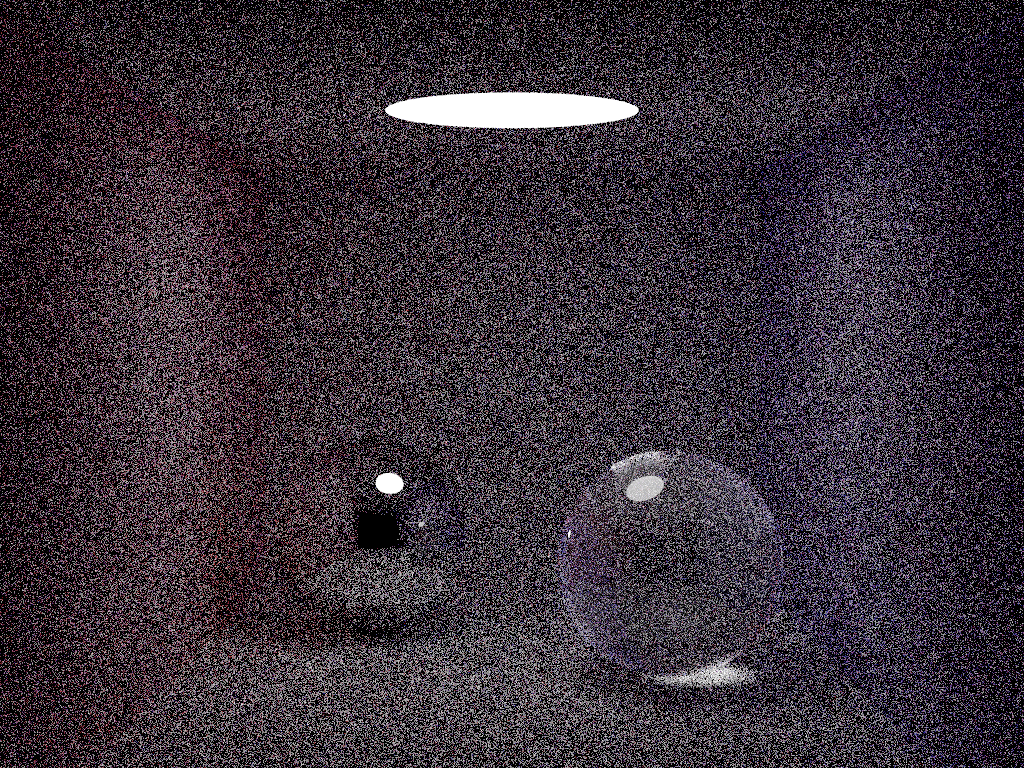
\includegraphics[width=\linewidth]{../assets/appendixD_result_8.png}
	\caption{8 campioni per pixel}
    \end{subfigure}\hspace{12pt}
    \begin{subfigure}[c]{0.4\linewidth}
	\centering
	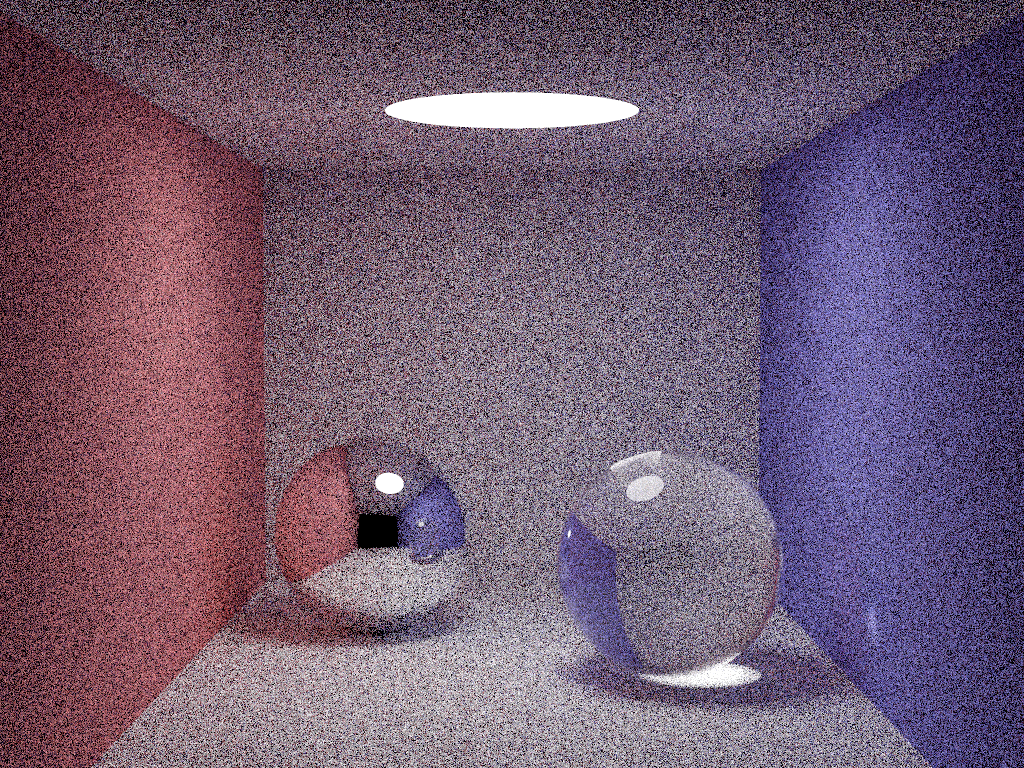
\includegraphics[width=\linewidth]{../assets/appendixD_result_40.png}
	\caption{40 campioni per pixel}
    \end{subfigure}\hfill
    \begin{subfigure}[c]{0.4\linewidth}
	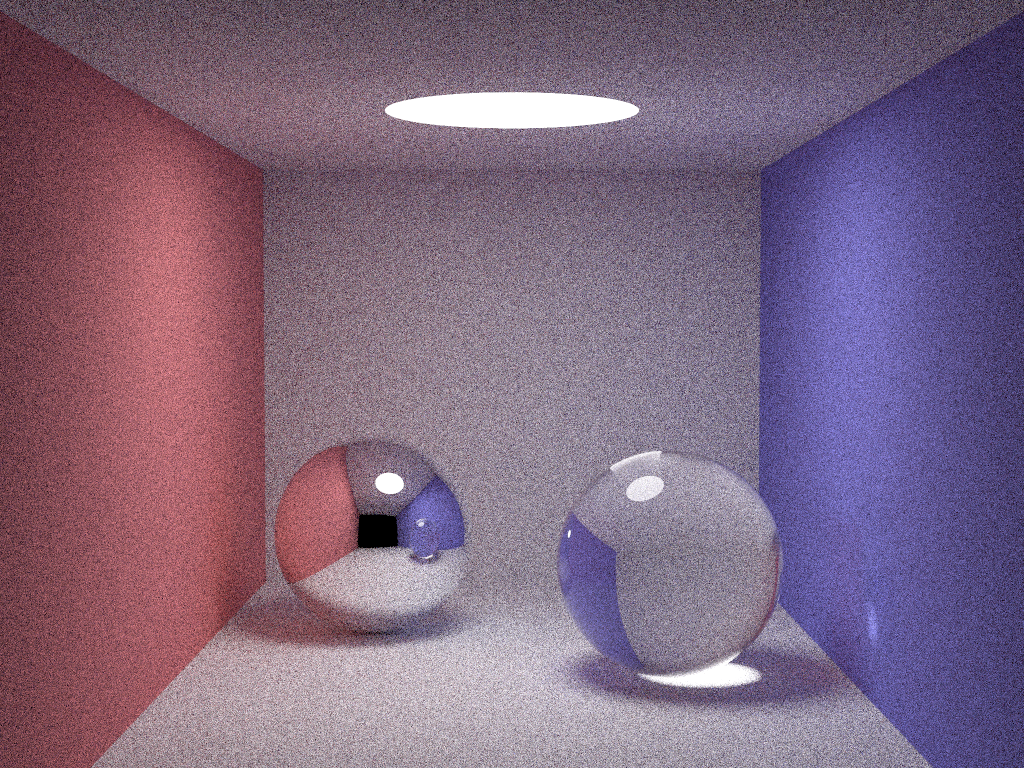
\includegraphics[width=\linewidth]{../assets/appendixD_result_200.png}
	\caption{200 campioni per pixel}
    \end{subfigure}\hfill
    \begin{subfigure}[c]{0.4\linewidth}
	\centering
	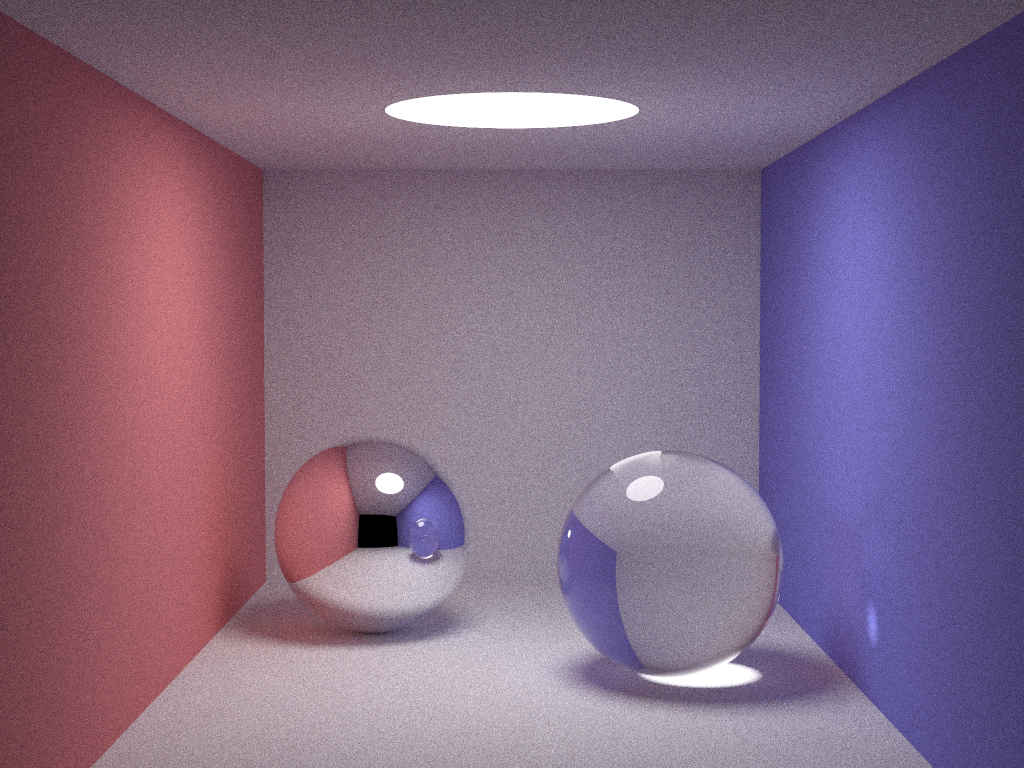
\includegraphics[width=\linewidth]{../assets/appendixD_result_1000.png}
	\caption{1000 campioni per pixel}
    \end{subfigure}\hfill
    \begin{subfigure}[c]{0.4\linewidth}
	\centering
	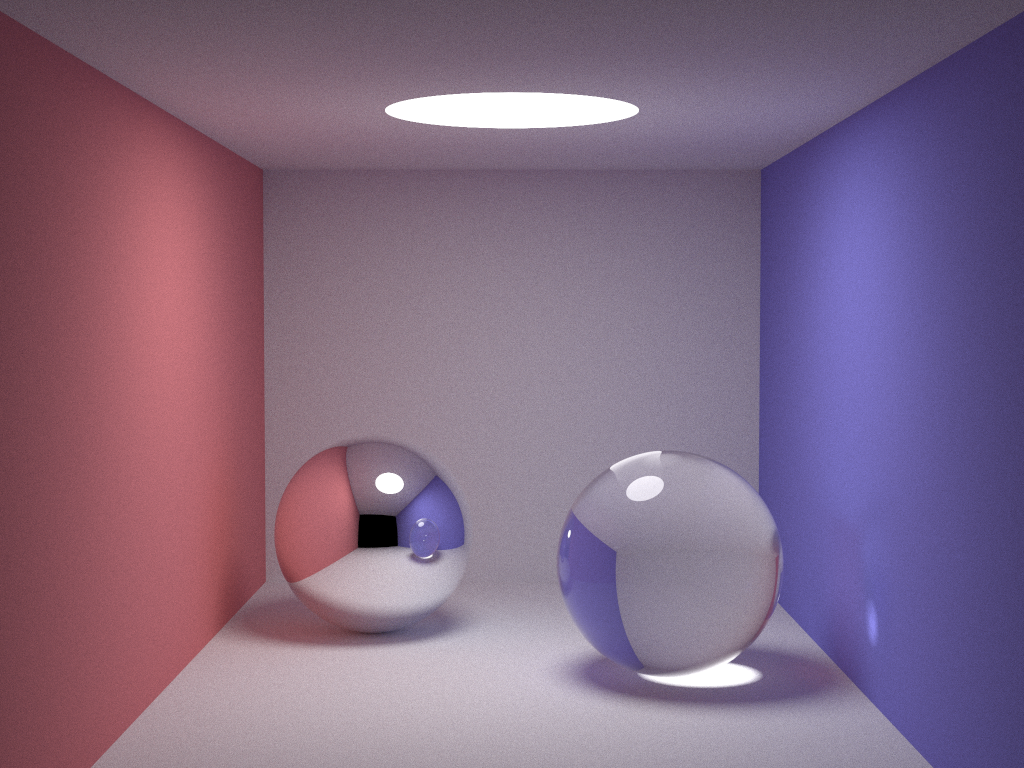
\includegraphics[width=\linewidth]{../assets/appendixD_result_5k.png}
	\caption{5000 campioni per pixel}
    \end{subfigure}\hfill
    \begin{subfigure}[c]{0.4\linewidth}
	\centering
	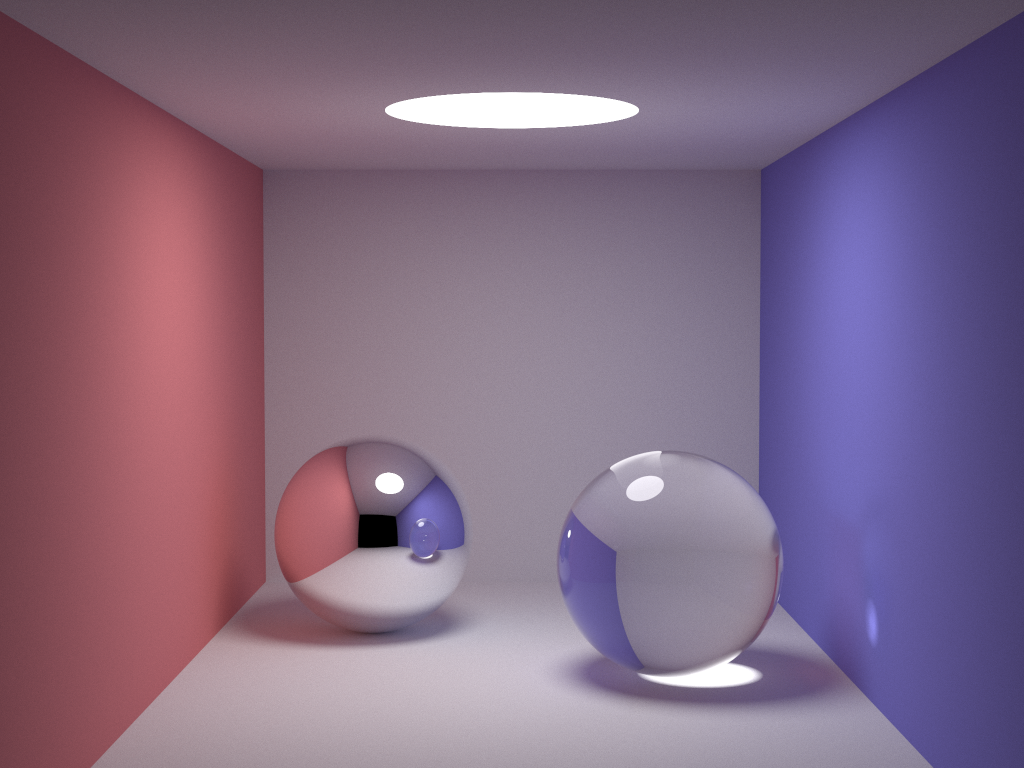
\includegraphics[width=\linewidth]{../assets/appendixD_result_25k.png}
	\caption{25000 campioni per pixel}
    \end{subfigure}
    \caption{Risultati dell'esecuzione dell'algoritmo con numero crescente di campioni per pixel}
\end{figure}
Comandi per la compilazione e resa (linux):
\begin{verbatim*}
g++ -O3 -fopenmp smallpt.cpp -o smallpt 
time ./smallpt 5000
display image.ppm
\end{verbatim*}
